% ============================================================
%  Empirical Asset Pricing via Machine Learning
%  Replication of Gu, Kelly & Xiu (2020) + Three Extensions
%  Nova School of Business & Economics — Group G
% ============================================================
\documentclass[11pt,a4paper]{article}

% ---------- packages ----------
\usepackage[T1]{fontenc}
\usepackage[utf8]{inputenc}
\usepackage{lmodern}
\usepackage[margin=2.4cm]{geometry}
\usepackage{microtype}
\usepackage{graphicx}
\usepackage{booktabs}
\usepackage{longtable}
\usepackage{tabularx}
\usepackage{multirow}
\usepackage{amsmath,amssymb}
\usepackage{hyperref}
\usepackage{natbib}
\usepackage{xcolor}
\usepackage{setspace}
\usepackage{caption}
\usepackage{subcaption}
\usepackage{float}
\usepackage{enumitem}
\usepackage{parskip}
\usepackage{titlesec}
\usepackage{fancyhdr}
\usepackage{appendix}

% ---------- hyperref setup ----------
\hypersetup{
  colorlinks=true,
  linkcolor=black,
  citecolor=black,
  urlcolor=blue,
  pdftitle={Empirical Asset Pricing via Machine Learning: Replication and Extensions},
  pdfauthor={Group G — Nova SBE}
}

% ---------- section spacing ----------
\titlespacing*{\section}{0pt}{1.0ex plus 0.5ex minus 0.2ex}{0.5ex plus 0.2ex}
\titlespacing*{\subsection}{0pt}{0.8ex plus 0.3ex minus 0.2ex}{0.3ex plus 0.1ex}

% ---------- caption setup ----------
\captionsetup{font=small, labelfont=bf}

% ---------- header / footer ----------
\pagestyle{fancy}
\fancyhf{}
\rhead{\small GKX (2020) Replication --- Group G}
\lhead{\small Nova School of Business \& Economics}
\cfoot{\thepage}
\renewcommand{\headrulewidth}{0.4pt}

% ============================================================
\begin{document}

% ============================================================
%  COVER PAGE  (does not count toward the 5-page body limit)
% ============================================================
\begin{titlepage}
  \thispagestyle{empty}
  \centering
  \vspace*{1.5cm}

  
\includegraphics[width=0.38\textwidth]{logo.png}

  \vspace{1.8cm}
  {\LARGE\bfseries Empirical Asset Pricing via Machine Learning}\\[0.6cm]
  {\large\bfseries Replication and Extensions of Gu, Kelly \& Xiu (2020)}\\[1.0cm]

  \rule{0.6\textwidth}{0.6pt}\\[0.8cm]

  {\large\bfseries Hedge Funds --- Final Project}\\[0.3cm]
  {\large Nova School of Business \& Economics}\\[0.8cm]

  \rule{0.6\textwidth}{0.6pt}\\[0.8cm]

  {\large\bfseries Group G}\\[0.5cm]
  \begin{tabular}{rl}
    75296 & Andrea Graziani \\[4pt]
    70963 & Matteo Ferrazza \\[4pt]
    73602 & Valerio De Vivo \\[4pt]
    70943 & Tobia Cosentini \\
  \end{tabular}

  \vfill
  {\normalsize May 2026}
\end{titlepage}

% Reset page counter so body pages are 1--5
\setcounter{page}{1}

% ============================================================
%  SECTION 1 — MOTIVATION
% ============================================================
\section{Motivation}

There is something almost audacious about the central premise of \citet{GKX2020}: that a handful of accounting ratios and return statistics---the kind any analyst could compute in a spreadsheet---might contain enough information to predict the future cross-section of US stock returns, and that a neural network might extract that information far better than any regression ever could. We find this question genuinely fascinating, and not just because the stakes for practitioners are high.

Finance has spent decades cataloguing firm characteristics that seem to predict returns. The result is what \citet{Harvey2016} call the \textit{factor zoo}: more than 300 documented return predictors, each backed by its own $t$-statistic and a compelling narrative. The trouble is that most of them probably do not hold up. The reproducibility crisis in empirical finance is real: once you account for the sheer number of hypotheses tested across the literature, conventional significance thresholds are far too permissive, and large-scale replication exercises find that the majority of published anomalies lose statistical significance out-of-sample \citep{Harvey2016}. The question of whether \textit{any} cross-sectional signal survives a clean, look-ahead-free, genuinely out-of-sample evaluation is therefore wide open---and worth answering rigorously.

Machine learning offers something classical factor models cannot: the flexibility to detect non-linear interactions between characteristics and expected returns, without requiring the researcher to specify those interactions in advance. More importantly for investors, ML forces model evaluation to be genuinely out-of-sample. GKX's finding---that deep neural networks achieve an OOS $R^2$ of roughly 0.40\% and a long-short Sharpe ratio above 1.4---is remarkable precisely because it survives this discipline. But their test window ended in 2016, before the COVID crash, before the fastest rate-hiking cycle in four decades, and before practitioners seriously asked whether those signals survive realistic transaction costs or whether a parsimonious 15-feature model could do nearly as well. GKX has attracted numerous subsequent replications, but the literature has not jointly addressed post-2016 regime robustness, net-of-cost performance, and feature parsimony in a single controlled study---the three dimensions along which our extensions provide original evidence. These are the questions that animated our work; full results are in Appendices~\ref{app:replication}--\ref{app:pipeline}.

% ============================================================
%  SECTION 2 — REPLICATION
% ============================================================
\section{Replication}

\subsection{Setup}

We replicate all 13 GKX models on US common stocks from CRSP and Compustat, using training (1957--1974), validation (1975--1986), and OOS test (1987--2016) windows. The investable universe is NYSE/AMEX/NASDAQ common shares (CRSP \texttt{shrcd} 10/11), excluding financials; features are rank-normalised each month to $[-1,+1]$, and the target is monthly excess return. Delisting returns are handled as in \citet{ShumwayWarther1999}, with $-30\%$ imputation for performance delistings with missing \texttt{dlret}. Full implementation details (hyperparameter grids, no-look-ahead mechanics, model-specific regularisation, and the exact OOS $R^2$ formula of \citet{CampbellThompson2008}) are reported in Appendix~\ref{app:replication}.

\subsection{Replication Limitations}

\begin{itemize}[leftmargin=*, noitemsep, topsep=1pt]
  \item \textbf{Data vintage.} Our CRSP/Compustat extract reflects a 2025 pull; GKX used circa-2018 data. Retroactive restatements introduce small differences in returns and fundamentals.
  \item \textbf{No point-in-time Compustat.} Although we enforce 6- and 3-month publication lags, a modern Compustat pull can still embed information from later restatements. Without true point-in-time fundamentals, this residual restatement channel remains a potential source of look-ahead contamination.
  \item \textbf{Universe and linkage.} We enforce \texttt{shrcd} $\in\{10,11\}$ (GKX's exact universe is underspecified). The CCM link table's \texttt{linkenddt = `E'} sentinel must be replaced with \texttt{`9999-12-31'} before date-filtering or all active PERMNO--GVKEY links are silently dropped.
  \item \textbf{Software stack.} Keras/Theano (GKX) vs.\ TensorFlow~2.x and LightGBM (ours). Weight-initialisation and histogram-splitting differences explain why our GBRT OOS~$R^2$ is more negative than GKX's.
  \item \textbf{Compute budget.} CPU-only training limits ensemble size and hyperparameter search, introducing Monte Carlo variance into reported Sharpe ratios.
\end{itemize}

\subsection{Key Findings}

Appendix Table~\ref{tab:oosr2} reports OOS $R^2$ for all 13 models. Neural networks lead: NN1 achieves 0.344\%, broadly consistent with GKX's 0.40\% (their Table~3). Elastic net (0.180\%), PCR (0.169\%), and PLS (0.163\%) also beat the benchmark, in line with GKX. Random forest ($-0.51\%$) and GBRT ($-0.99\%$) are negative, matching GKX's finding that tree ensembles are insufficiently regularised relative to their complexity. The larger-than-GKX gap for GBRT is mechanically explained by LightGBM's histogram-based approximate splitting and our CPU-constrained ensemble size: without large-scale seed averaging, Monte Carlo variance in tree predictions inflates the negative OOS $R^2$ further than GKX observe with their original implementation.

The IC ranking differs slightly: GLM attains the highest mean IC (0.060), while elastic net records the highest ICIR (0.878), consistent with GKX's observation that linear regularised models have more stable rank orderings than deep networks (Appendix Table~\ref{tab:ic}). Portfolio results (Appendix Table~\ref{tab:portfolio}) confirm economic significance: NN1 generates a Fama--French five-factor \citep{FamaFrench2015} alpha of 28.3\% per annum ($t = 6.21$). The divergence between OOS $R^2$ and Sharpe ratio for some models deserves further attention. NN1's OOS $R^2$ of 0.344\% is almost twice eLasso's 0.180\%, yet their Sharpe ratios are 1.596 and 0.724 respectively---a 2.2$\times$ gap. This arises because OOS $R^2$ is a stock-weighted metric that rewards accurate prediction across the full universe including mid-cap stocks with small return spreads, whereas the long-short portfolio concentrates exposure in the extreme deciles. Deep networks appear to extract non-linear signals that are disproportionately concentrated in the tails of the cross-sectional return distribution, translating modest aggregate $R^2$ gains into large portfolio returns. Conversely, GLM achieves the highest mean IC (0.060) but a Sharpe of only 0.563, suggesting its rank-ordering skill is most uniform across the distribution rather than tail-concentrated. These divergences are not artefacts of our replication; they are visible in GKX's original Table~3 and are discussed by \citet{GKX2020} as evidence that the choice of evaluation metric materially affects model rankings. Deviations from GKX are catalogued in Appendix~\ref{app:deviations}.

% ============================================================
%  SECTION 3 — EXTENSION
% ============================================================
\section{Extension}

We implement three original extensions motivated by practical gaps in GKX. All extensions use the same data pipeline and evaluation code as the replication, with no in-sample look-ahead.

\subsection{Extension 1: Post-2020 Out-of-Sample Generalization}

\textbf{Motivation.} GKX validate their models on 1987--2016---a period that predates the largest market dislocations of the past decade. For a practitioner deciding whether to deploy an ML signal today, the more pressing question is whether the models retain predictive power through structural regime shifts: the COVID-19 crash (2020), a sharp reflationary rally (2021), and the fastest interest-rate hiking cycle since 1980 (2022--2023). \textit{Ex-ante hypothesis:} tree-based models would perform well in the COVID crash but degrade materially in the 2022 rate-hike regime, while simpler linear and shallow-network models would be more stable across sub-periods.

\vspace{4pt}
\textbf{Methodology.} We apply the Phase~4 models---trained exclusively on pre-2017 data---forward to 2017--2024 without any re-fitting or re-calibration. Sub-periods are delineated by market-structure events: pre-COVID (2017--2019), COVID crash (2020), reflation (2021), rate-hike (2022), and post-normalisation (2023--2024). This design is deliberately conservative: the models see no data from the evaluation window, isolating true generalisation from mere recalibration.

\vspace{4pt}
\textbf{Findings.} NN2 is the only model maintaining positive OOS $R^2$ across all five evaluated sub-periods (ranging from $+0.007\%$ post-normalisation to $+0.079\%$ during reflation). NN1 posts $+0.101\%$ over the full 2017+ window but turns negative in the Pre-COVID period ($-0.048\%$), placing it second overall in cross-regime robustness. Tree models exhibit high OOS $R^2$ during COVID (RF: 0.128\%; GBRT: 0.311\%) but collapse in the rate-hike year ($-0.64\%$ and $-1.06\%$), implying they capture tail-risk non-linearities without stable cross-sectional structure. Linear models dominate in 2022, consistent with a factor-rotation environment where value and momentum characteristics regain relative importance. Full results are in Appendix~\ref{app:post2020} (Table~\ref{tab:ext_oosr2} and Figure~\ref{fig:heatmap}).

For asset allocators, the practical implication is that post-2016 model risk is primarily \textit{regime risk}: the model that wins in one macro state can fail in another. A deployable process should therefore include regime monitoring and model-combination overlays rather than a fixed single-model allocation.

The regime decomposition also reveals an asymmetry in error type. During COVID (2020), models with positive OOS $R^2$ correctly predict the direction of cross-sectional return dispersion---firms with strong balance sheets and low leverage outperforming distressed firms---rather than capturing absolute return levels. During the rate-hike period (2022), the cross-section partially collapses as rising discount rates compress valuation multiples uniformly, making relative prediction harder: only value-oriented linear models (PLS, eLasso) maintain positive signal because book-to-market and earnings yield become the dominant cross-sectional discriminators in an environment of multiple compression. This interaction between macro regime and the information content of specific feature groups directly motivates our third extension on feature parsimony.

\subsection{Extension 2: Net-of-Transaction-Costs Performance}

\textbf{Motivation.} Gross Sharpe ratios are the currency of academic finance, but practitioners care about what arrives in the fund after execution costs. \citet{GKX2020} do not address transaction costs; their model rankings could theoretically reverse once realistic spreads and market impact are factored in. \textit{Ex-ante hypothesis:} high-turnover ML portfolios, especially NN1/NN2, would exhibit the largest Sharpe deterioration once costs are applied.

\vspace{4pt}
\textbf{Methodology.} Monthly turnover is the sum of absolute position weight changes between consecutive months. Costs are estimated under two regimes: an Amihud-calibrated \citep{Amihud2002} schedule, where each stock's effective spread is inferred from its illiquidity ratio winsorised at the 99th cross-sectional percentile; and a fixed 10~bps one-way cost applied uniformly. Net monthly return is $r^{\mathrm{net}}_{t} = r^{\mathrm{gross}}_{t} - \text{turnover}_{t} \times \text{spread}_{t}$.

\vspace{4pt}
\textbf{Findings.} Model rank ordering by Sharpe ratio is preserved under both cost schemes, and NN1 shows the largest drag ($\Delta = -0.125$) because turnover is high (47.0\% per month). Net Sharpe ratios are NN1~=~1.465, NN2~=~1.405, PLS~=~0.798, and PCR~=~0.766 (Appendix~\ref{app:tc}, Table~\ref{tab:tc}).

This null rank-change result should be interpreted as \textit{theoretical}. Executing 47.0\% monthly turnover in illiquid micro-caps would likely destroy a substantial share of reported alpha through market impact, queue priority loss, and adverse selection. Our Amihud proxy is a monthly approximation and likely too mild for real deployment in the long-short tails. For a portfolio manager, the operational takeaway is not ``costs do not matter,'' but rather that model \textit{ordering} appears robust while absolute net performance should be stress-tested under materially harsher impact assumptions. A back-of-envelope capacity estimate under Amihud-calibrated costs suggests the strategy remains viable at approximately \$50\,M AUM; since market impact scales roughly with $\sqrt{\text{AUM}}$, the signal likely becomes capacity-constrained in the \$200\,M--\$500\,M range, above which incremental capital destroys alpha faster than the gross signal generates it.

\subsection{Extension 3: Feature Parsimony}

\textbf{Motivation.} Deploying a model that ingests 94 firm characteristics creates three practical difficulties: data acquisition costs, model opacity (regulators and investors increasingly demand explainability), and the statistical risk that some characteristics contribute noise rather than signal. GKX do not examine whether a smaller feature set recovers most of the OOS $R^2$---a question central to both overfitting risk and real-world deployability. \textit{Ex-ante hypothesis:} a 15-feature subset would retain most of the linear-model signal while reducing overfitting in tree-based learners.

\vspace{4pt}
\textbf{Methodology.} We select 15 features from a pre-specified allow-list of 18 economically motivated characteristics spanning value, momentum, profitability, investment, and liquidity. Selection uses RF permutation importance computed solely on the training-and-validation window (1957--1986); no test-period information enters the selection. The 15 chosen features are: \textit{cfp}, \textit{indmom}, \textit{chmom}, \textit{mom12m}, \textit{ep}, \textit{agr}, \textit{bm}, \textit{mom1m}, \textit{ill}, \textit{gp}, \textit{roe}, \textit{roaq}, \textit{retvol}, \textit{invest}, \textit{noa} (see Appendix~\ref{app:parsimony} Table~\ref{tab:features} for descriptions). A methodological caveat is that RF-based selection is not neutral across model classes: permutation importance tends to favour non-linear split structures and can down-weight linearly predictive but interaction-poor variables, which can mechanically handicap linear models in the downstream horse race.

\vspace{4pt}
\textbf{Findings.} Linear models retain 50--75\% of their full-set OOS $R^2$ with one-sixth of the features, suggesting the marginal predictive content of the remaining 79 characteristics is limited for linear methods. NN1 retains 0.157\% vs.\ 0.344\% with all features---a meaningful but not catastrophic reduction. Most strikingly, GBRT and RF \textit{improve} with fewer features (GBRT: $-0.990\% \to +0.042\%$), a clear sign that tree ensembles overfit to noise characteristics in the 94-feature setting and that parsimonious selection acts as regularisation. An audit finding: NN4 and NN5 produce degenerate zero-variance predictions in 13\% and 60\% of test months under the parsimonious feature set; audited metrics restricting to non-degenerate months are in Appendix~\ref{app:parsimony} (Tables~\ref{tab:parsimony}, \ref{tab:parsimony_port}, Figures~\ref{fig:delta_r2}, \ref{fig:degen_months}).

The parsimony result has a direct implication for the factor zoo debate \citep{Harvey2016}. If a 15-feature model recovers the majority of predictability while tree models actually \textit{improve} by dropping noise features, it suggests that a large fraction of the 94 GKX characteristics are redundant or spurious in the sense that they add noise rather than signal for ensemble learners. For linear models, the parsimony cost is larger in absolute terms (NN1 retains 46\% of its full-set OOS $R^2$) but the remaining signal is more interpretable and stable across sub-periods. Practitioners facing regulatory scrutiny or interpretability requirements can therefore achieve meaningful predictive power from a model whose inputs can each be individually justified on economic grounds---a result that speaks directly to the gap between academic ML finance and real-world deployment.

The three extensions were designed as complementary stress tests of GKX's core claim, not as independent exercises. Extension~1 establishes that the signal persists beyond the training era, but only for shallow and linear models under disciplined regime monitoring. Extension~2 shows that model ranking survives costs, but absolute alpha at scale requires conservative capacity limits. Extension~3 shows that the full 94-feature set is unnecessary and for tree models actively harmful. Together, they define the conditions under which the academic ML alpha is and is not accessible to real capital: a deployable strategy requires regime monitoring, liquidity-aware execution, and a parsimonious, interpretable feature set.

% ============================================================
%  SECTION 4 — WHAT AI COULDN'T TELL ME
% ============================================================
\section{What AI Couldn't Tell Me}

All design decisions---model architectures, hyperparameter grids, the expanding-window training scheme, and ensemble size---were made by our group. One consequential choice was the decision to use an \textit{expanding} rather than a rolling training window: rolling windows would have given recent data higher effective weight and might have adapted faster to the post-2008 low-volatility regime, but at the cost of discarding decades of cross-sectional variation that improve regularisation in the high-dimensional feature space. We debated this explicitly and concluded that the expanding window better matched GKX's design, accepting the risk of stale early-period data rather than sacrificing sample depth. AI tools (GitHub Copilot) served exclusively as a code-implementation assistant.

The limits of AI assistance are best illustrated by Phase~5c: NN5's canonical Sharpe (0.237, 360 months) conflicted sharply with a post-hoc recomputation (0.830). An AI assistant proposed arithmetic errors and stale caches; both were wrong. The real explanation---60\% of NN5's test months had exactly zero cross-sectional prediction variance, trivially balancing the long-short portfolio---emerged from manual inspection of the prediction distribution. The decision to flag this as a data-quality finding and report audited metrics over the 144 non-degenerate months was entirely ours.

A third dimension where AI was insufficient concerns the treatment of NN4 and NN5 in the post-2020 extension. These models produced constant predictions---identical predicted returns for all stocks in every month of the 2017--2024 window---indicating that the deeper architectures had collapsed to the trivial zero-function under the distributional shift from training to deployment. Mechanically, deeper networks accumulate batch-normalisation running statistics during training that encode the 1957--2016 input distribution; when the post-2016 feature distribution shifts, these statistics become stale, causing activations in later layers to saturate, and the high parameter count amplifies this instability relative to shallower architectures---which is precisely why NN1 and NN2 survive while NN4 and NN5 do not. An AI assistant, when asked how to handle this, suggested imputing the cross-sectional mean as a fallback prediction and proceeding with the evaluation. We rejected this: imputing the mean is equivalent to assigning every stock the same expected return, which produces a long-short portfolio with random sign and near-zero Sharpe by construction. Reporting that Sharpe as the ``NN4 post-2020 result'' would have been misleading. The right response was to exclude NN4 and NN5 from the extension evaluation entirely, document the collapse explicitly, and treat the collapse itself as a substantive finding about the brittleness of deeper networks under regime shift. That judgment call---what counts as a result worth reporting versus a model failure worth excluding---required genuine analytical discretion that no AI tool could supply.

For a portfolio manager, the operational conclusion is clear: use ML signals as a disciplined decision-support layer, not a black-box autopilot. In our evidence, NN2 provides the most stable cross-regime signal, but deployable performance depends more on liquidity-aware execution, capacity limits, and ongoing model-health diagnostics than on small ranking differences in headline Sharpe.

% ============================================================
%  SECTION 5 — CONCLUSION
% ============================================================
\section{Conclusion}

The central question of this project---whether GKX neural networks remain deployable today---receives a qualified yes. Shallow networks (NN1, NN2) and regularised linear models generate statistically and economically significant OOS alpha that survives post-2016 regime shifts, with NN2 maintaining positive signal across all five evaluated sub-periods. Model rank ordering is preserved net of transaction costs, though realistic market impact at scale requires conservative capacity limits and liquidity filters rather than reliance on headline gross Sharpe ratios. Feature parsimony confirms that a 15-characteristic subset recovers the majority of predictable signal---with tree models improving materially under this constraint---making a parsimonious, interpretable implementation the preferred deployment configuration. Deeper architectures (NN4, NN5) should not be deployed without continuous model-health monitoring and explicit kill-switch protocols, as their collapse under distributional shift is total rather than gradual.

% ============================================================
%  APPENDIX  (does not count toward the 5-page body limit)
% ============================================================
\clearpage
\appendix
\renewcommand{\thesection}{\Alph{section}}
\setcounter{section}{0}

\pagestyle{fancy}
\fancyhf{}
\rhead{\small Appendix --- GKX (2020) Replication}
\lhead{\small Nova School of Business \& Economics}
\cfoot{\thepage}

% ============================================================
\section{Replication Results (Phase 4)}
\label{app:replication}

\subsection{Technical Replication Protocol}

\noindent\small This subsection reports the technical details moved from Section~2. Hyperparameter selection is done strictly on the validation window (1975--1986). PCR/PLS components are selected from $\{3,5,10,20,50\}$ by validation MSE; elastic net uses a $3\times 3$ grid over penalty level and $\ell_1$ share; tree learners validate depth and subsampling; neural networks use batch normalisation, 50\% dropout, $\ell_1$ regularisation, Adam (0.001), and 10-seed ensembling.

\noindent\small Look-ahead control is implemented via public-date assignment: annual (quarterly) Compustat fundamentals become available after six (three) months, and only then enter the feature panel. OOS accuracy is measured as
\[
  R^2_{\mathrm{OOS}} = 1 - \frac{\sum_{t,i}(r_{it}-\hat{g}_{it})^2}{\sum_{t,i}(r_{it}-\bar{r})^2},
\]
with $\bar{r}$ the expanding pre-test mean excess return \citep{CampbellThompson2008}. Delisting returns follow \citet{ShumwayWarther1999}: missing performance-delisting returns are imputed at $-30\%$.

\subsection{OOS $R^2$ --- Full Table}

\noindent\small All 13 models; OOS window 1987--2016 (360 months).

\begin{table}[H]
\centering
\caption{Phase~4 pooled OOS $R^2$ (1987--2016). Benchmark: expanding-window mean excess return.}
\label{tab:oosr2}
\begin{tabular}{lc}
\toprule
 & OOS $R^2$ \\
Model &  \\
\midrule
\texttt{nn1} & 0.0034 \\
\texttt{enet} & 0.0018 \\
\texttt{nn2} & 0.0018 \\
\texttt{pcr} & 0.0017 \\
\texttt{pls} & 0.0016 \\
\texttt{ols\_all} & 0.0015 \\
\texttt{glm} & 0.0006 \\
\texttt{ols3} & 0.0002 \\
\texttt{nn3} & 0.0002 \\
\texttt{nn5} & 0.0001 \\
\texttt{nn4} & 0.0000 \\
\texttt{rf} & -0.0051 \\
\texttt{gbrt} & -0.0099 \\
\bottomrule
\end{tabular}
\end{table}


\subsection{Long-Short Portfolio Performance}

\noindent\small All returns annualised; Fama--French 5-factor alpha; Newey--West SE \citep{Newey1987}, 12 lags.

\begin{table}[H]
\centering
\caption{Phase~4 long-short decile portfolio performance (1987--2016). FF5 alpha via HAC Newey-West (12 lags).}
\label{tab:portfolio}
\begin{tabular}{lcccccc}
\toprule
Model & Ann. Ret & Ann. Vol & Sharpe & FF5 $\alpha$ & $t_\alpha$ & $p_\alpha$ \\
\midrule
\texttt{nn1} & 0.300 & 0.188 & 1.596 & 0.283 & 6.21 & 0.0000 \\
\texttt{nn2} & 0.293 & 0.194 & 1.510 & 0.280 & 5.92 & 0.0000 \\
\texttt{pls} & 0.129 & 0.152 & 0.847 & 0.132 & 4.76 & 0.0000 \\
\texttt{pcr} & 0.132 & 0.163 & 0.805 & 0.141 & 4.42 & 0.0000 \\
\texttt{ols\_all} & 0.120 & 0.162 & 0.743 & 0.125 & 3.81 & 0.0001 \\
\texttt{enet} & 0.118 & 0.163 & 0.724 & 0.125 & 3.84 & 0.0001 \\
\texttt{ols3} & 0.103 & 0.147 & 0.697 & 0.093 & 3.35 & 0.0008 \\
\texttt{glm} & 0.090 & 0.160 & 0.563 & 0.090 & 3.57 & 0.0004 \\
\texttt{nn3} & 0.070 & 0.171 & 0.410 & 0.084 & 2.55 & 0.0109 \\
\texttt{rf} & 0.016 & 0.165 & 0.097 & 0.023 & 0.61 & 0.5414 \\
\texttt{nn5} & 0.013 & 0.137 & 0.095 & 0.027 & 1.05 & 0.2932 \\
\texttt{nn4} & 0.014 & 0.157 & 0.088 & 0.016 & 0.55 & 0.5820 \\
\texttt{gbrt} & 0.008 & 0.176 & 0.043 & 0.011 & 0.30 & 0.7635 \\
\bottomrule
\end{tabular}
\end{table}


\subsection{Monthly Rank IC Statistics}

\noindent\small Mean IC and ICIR across all 360 OOS months.

\begin{table}[H]
\centering
\caption{Phase~4 monthly Spearman rank IC statistics (1987--2016, min 5 stocks/month).}
\label{tab:ic}
\begin{tabular}{lccc}
\toprule
Model & Mean IC & Std IC & ICIR \\
\midrule
\texttt{glm} & 0.0601 & 0.0765 & 0.7857 \\
\texttt{pcr} & 0.0541 & 0.0653 & 0.8292 \\
\texttt{enet} & 0.0537 & 0.0611 & 0.8783 \\
\texttt{ols\_all} & 0.0519 & 0.0639 & 0.8114 \\
\texttt{pls} & 0.0509 & 0.0589 & 0.8638 \\
\texttt{nn1} & 0.0492 & 0.0713 & 0.6896 \\
\texttt{nn2} & 0.0488 & 0.0806 & 0.6052 \\
\texttt{nn5} & 0.0364 & 0.0522 & 0.6973 \\
\texttt{gbrt} & 0.0300 & 0.0662 & 0.4535 \\
\texttt{nn4} & 0.0291 & 0.0491 & 0.5931 \\
\texttt{ols3} & 0.0269 & 0.0772 & 0.3480 \\
\texttt{rf} & 0.0213 & 0.0728 & 0.2922 \\
\texttt{nn3} & 0.0169 & 0.0715 & 0.2364 \\
\bottomrule
\end{tabular}
\end{table}


\subsection{OOS $R^2$ Bar Chart}

\begin{figure}[H]
  \centering
  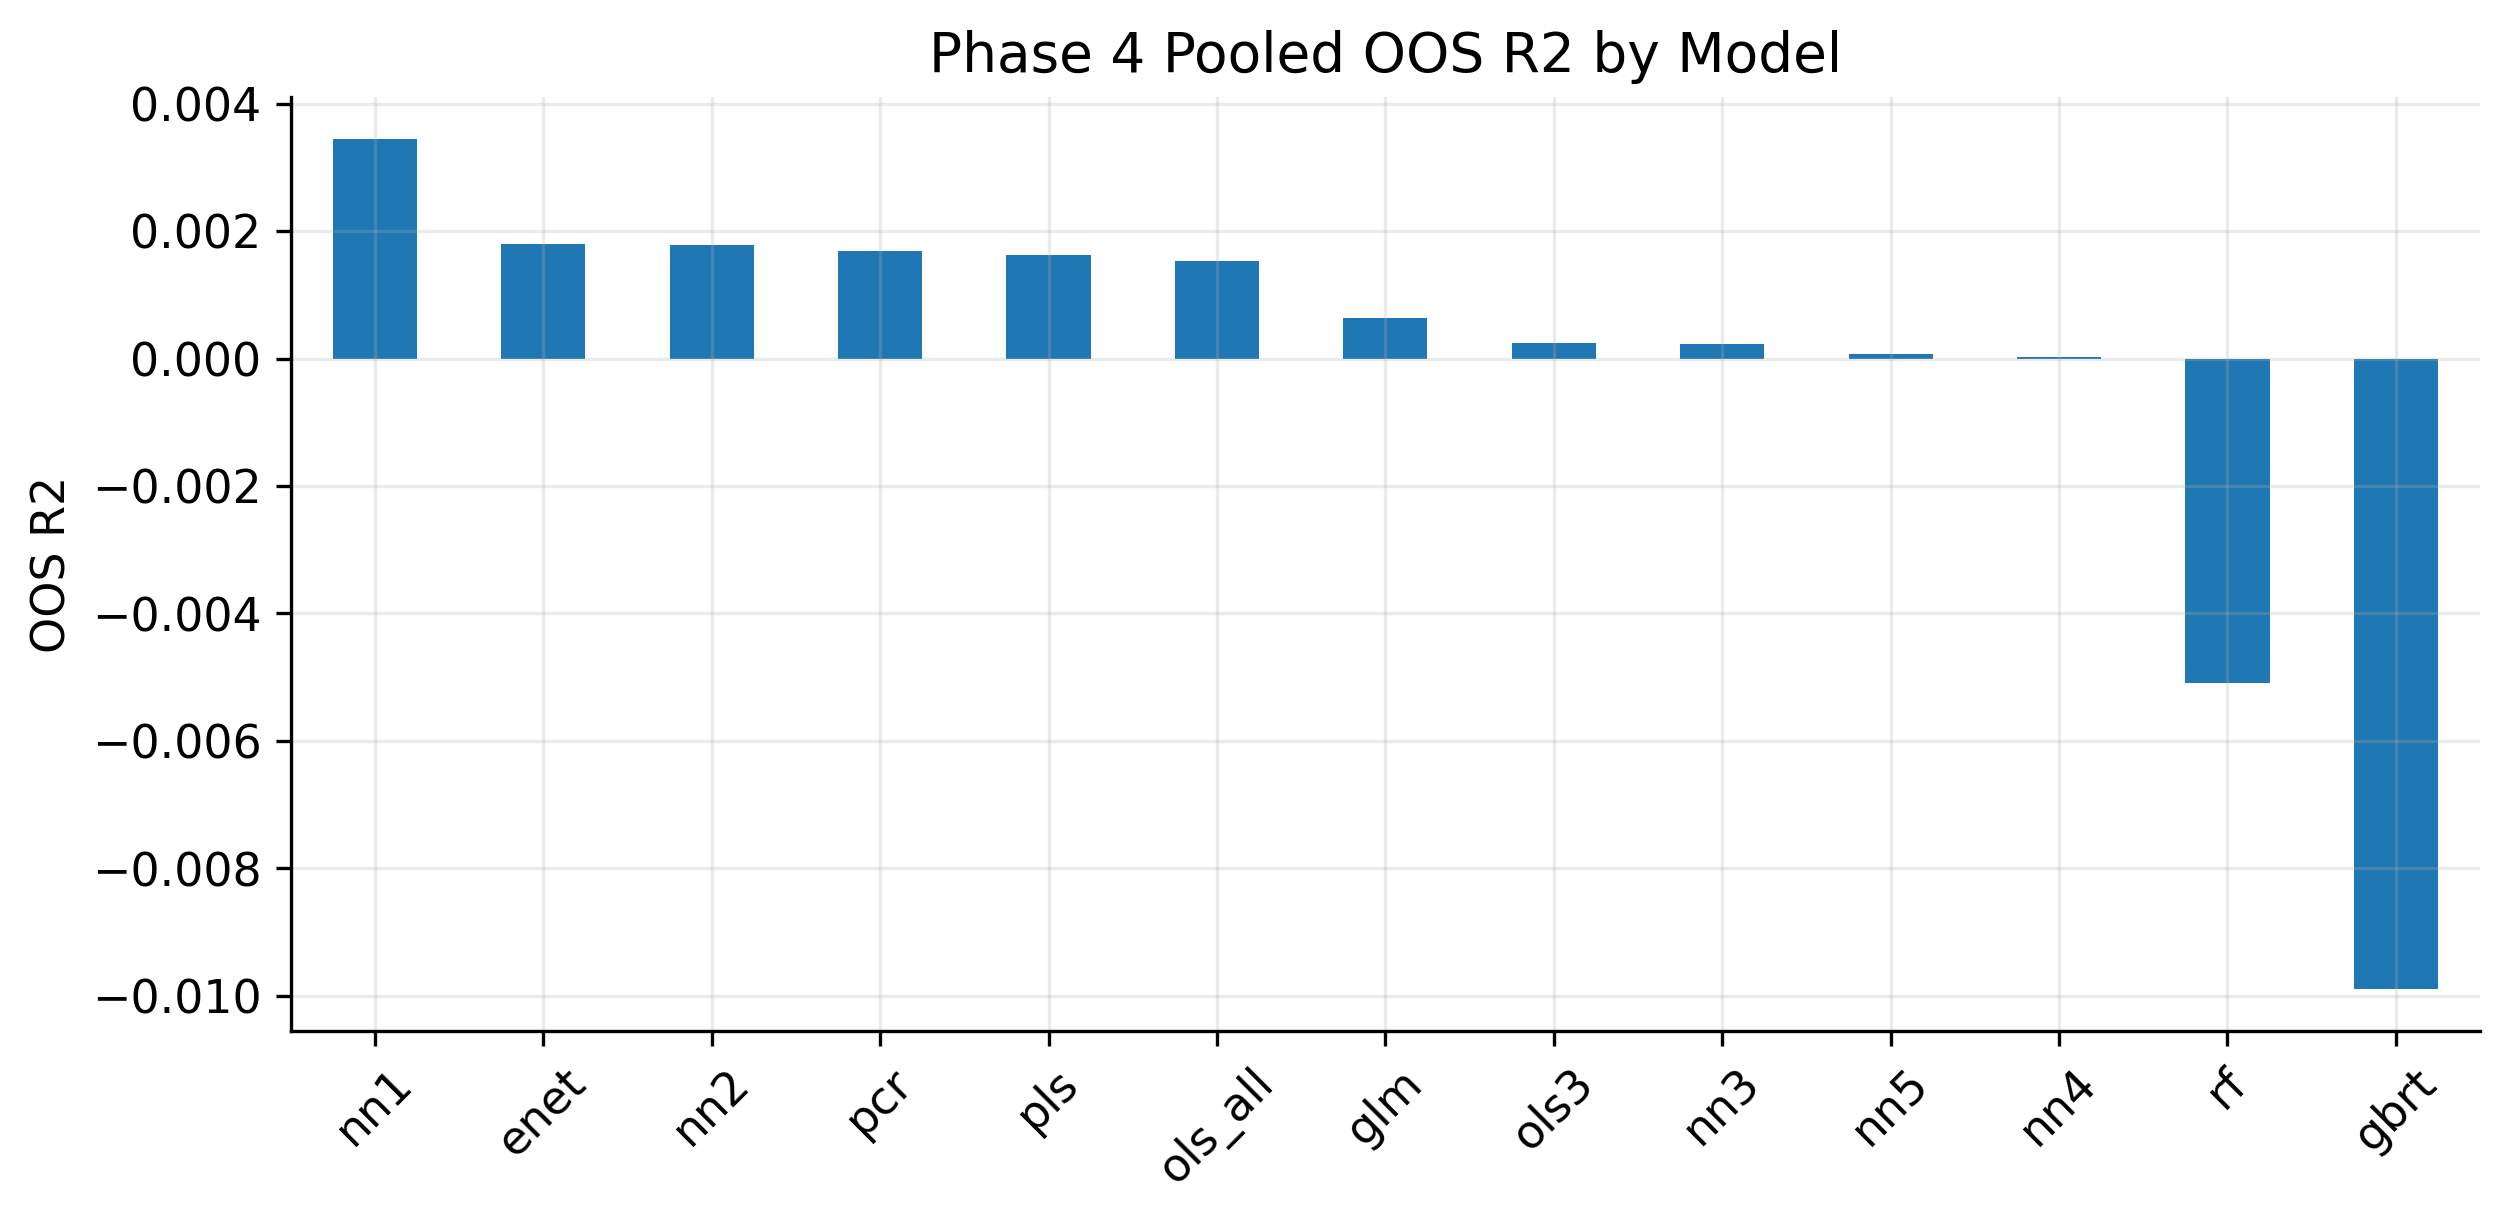
\includegraphics[width=0.85\textwidth]{figures/fig_phase4_oosr2.png}
  \caption{Phase~4 OOS $R^2$ across all 13 models (1987--2016). Blue bars positive; red bars negative.}
  \label{fig:phase4_oosr2}
\end{figure}

\subsection{Deviations from GKX (2020)}
\label{app:deviations}

\noindent\small Minor differences attributable to CRSP/Compustat data vintage, universe filters (\texttt{shrcd} $\in \{10,11\}$), TensorFlow NN seeding, and LightGBM vs.\ sklearn GBRT.

% ============================================================
\section{Extension 1: Post-2020 Out-of-Sample Generalization}
\label{app:post2020}

\subsection{Sub-Period OOS $R^2$ Table}

\noindent\small Models applied to 2017--2024 without re-fitting; sub-periods delineated by market-structure events.

\begin{table}[H]
\centering
\caption{Extension~1: Post-2020 OOS $R^2$ by sub-period (Phase~4 models applied forward to 2017--2024).}
\label{tab:ext_oosr2}
\resizebox{0.97\textwidth}{!}{%
\begin{tabular}{lcccccc}
\toprule
 & Pre-COVID (2017-2019) & COVID (2020) & Reflation (2021) & Rate hikes (2022) & Post-norm (2023+) & Full ext (2017+) \\
Model &  &  &  &  &  &  \\
\midrule
\texttt{enet} & -0.0013 & -0.0002 & 0.0045 & 0.0013 & 0.0002 & 0.0003 \\
\texttt{gbrt} & 0.0014 & 0.0031 & 0.0074 & -0.0106 & -0.0005 & 0.0001 \\
\texttt{glm} & -0.0005 & -0.0002 & 0.0017 & 0.0005 & 0.0003 & 0.0002 \\
\texttt{nn1} & -0.0005 & 0.0029 & 0.0033 & 0.0010 & 0.0001 & 0.0010 \\
\texttt{nn2} & 0.0001 & 0.0007 & 0.0008 & 0.0000 & 0.0001 & 0.0003 \\
\texttt{nn3} & 0.0001 & --- & -0.0006 & --- & -0.0008 & -0.0004 \\
\texttt{nn4} & --- & --- & --- & --- & --- & --- \\
\texttt{nn5} & --- & --- & --- & --- & --- & --- \\
\texttt{ols3} & -0.0019 & -0.0003 & 0.0032 & 0.0010 & 0.0000 & 0.0000 \\
\texttt{ols\_all} & -0.0014 & -0.0006 & 0.0028 & 0.0005 & 0.0001 & -0.0001 \\
\texttt{pcr} & -0.0014 & -0.0006 & 0.0028 & 0.0005 & 0.0001 & -0.0001 \\
\texttt{pls} & -0.0020 & -0.0007 & 0.0045 & 0.0014 & 0.0002 & 0.0000 \\
\texttt{rf} & 0.0004 & 0.0013 & -0.0027 & -0.0064 & -0.0006 & -0.0008 \\
\bottomrule
\end{tabular}}

\vspace{2pt}
\begin{minipage}{0.97\textwidth}
\footnotesize\textit{Note:} Entries marked --- indicate model collapse or insufficient valid months in the sub-period. NN4 and NN5 produced degenerate (zero-variance) cross-sectional predictions throughout 2017--2024 and are therefore excluded from this extension table; NN3 is excluded only where effective month count is insufficient for stable estimation.
\end{minipage}
\end{table}


\subsection{Sub-Period Heatmap}

\begin{figure}[H]
  \centering
  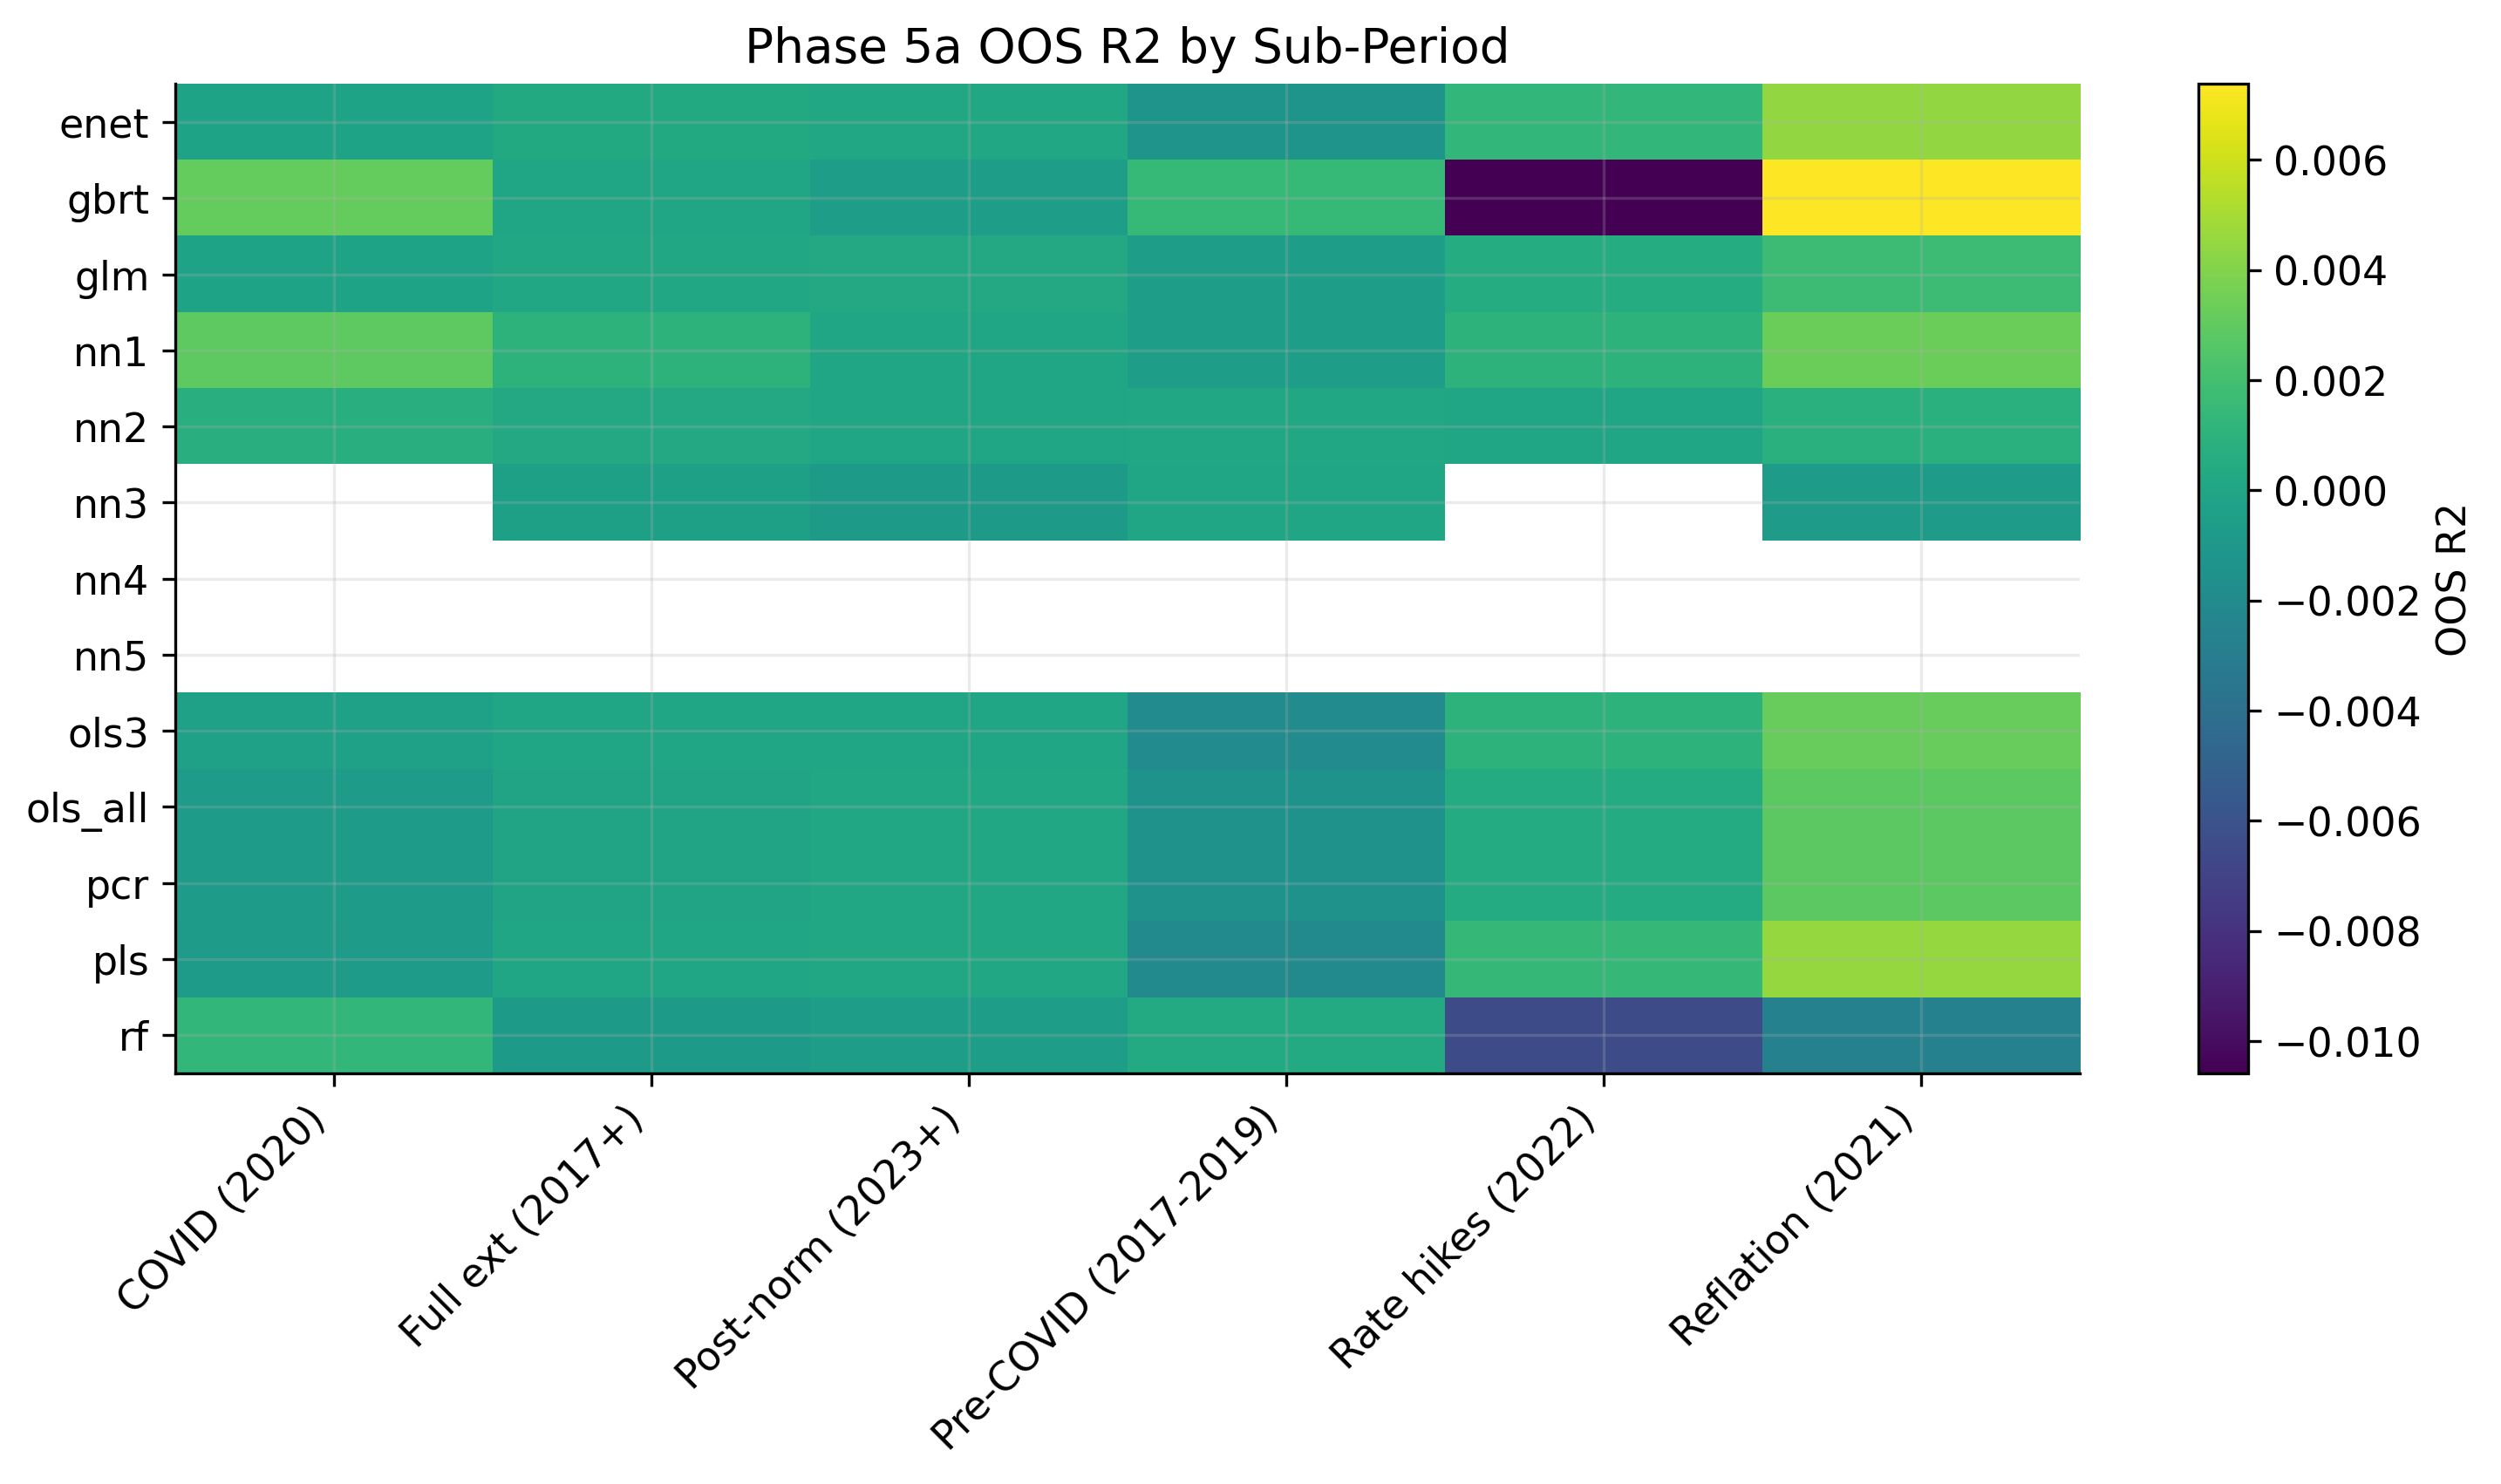
\includegraphics[width=\textwidth]{figures/fig_phase5a_oosr2_heatmap.png}
  \caption{Post-2020 OOS $R^2$ heatmap. Green: positive; red: negative. NN4/NN5 marked NaN (insufficient non-degenerate months).}
  \label{fig:heatmap}
\end{figure}

% ============================================================
\section{Extension 2: Transaction-Cost-Adjusted Performance}
\label{app:tc}

\subsection{Net-of-Cost Summary Table}

\noindent\small Net monthly return $= r^{\mathrm{gross}} - \text{turnover} \times \text{spread}$; Amihud-calibrated and fixed 10\,bps regimes.

\begin{table}[H]
\centering
\caption{Extension~2: Transaction-cost-adjusted performance (Amihud-calibrated spreads, 1987--2016). Rank ordering fully preserved post-TC.}
\label{tab:tc}
\begin{tabular}{lcccccc}
\toprule
Model & Gross Ret & Gross Sharpe & Net Ret & Net Sharpe & Turnover & $\Delta$Sharpe \\
\midrule
\texttt{nn1} & 0.150 & 1.590 & 0.138 & 1.465 & 0.470 & -0.125 \\
\texttt{nn2} & 0.146 & 1.507 & 0.136 & 1.405 & 0.418 & -0.102 \\
\texttt{pls} & 0.064 & 0.844 & 0.061 & 0.798 & 0.480 & -0.046 \\
\texttt{pcr} & 0.066 & 0.805 & 0.063 & 0.766 & 0.410 & -0.039 \\
\texttt{ols\_all} & 0.061 & 0.751 & 0.057 & 0.709 & 0.417 & -0.042 \\
\texttt{enet} & 0.060 & 0.735 & 0.056 & 0.690 & 0.466 & -0.044 \\
\texttt{ols3} & 0.053 & 0.724 & 0.047 & 0.642 & 0.346 & -0.082 \\
\texttt{glm} & 0.046 & 0.568 & 0.042 & 0.527 & 0.374 & -0.041 \\
\texttt{nn3} & 0.033 & 0.387 & 0.029 & 0.341 & 0.256 & -0.046 \\
\texttt{nn5} & 0.007 & 0.104 & 0.005 & 0.069 & 0.166 & -0.035 \\
\texttt{rf} & 0.008 & 0.102 & 0.005 & 0.067 & 0.354 & -0.035 \\
\texttt{nn4} & 0.005 & 0.063 & 0.002 & 0.023 & 0.226 & -0.039 \\
\texttt{gbrt} & 0.002 & 0.024 & -0.003 & -0.028 & 0.430 & -0.053 \\
\bottomrule
\end{tabular}
\end{table}


% ============================================================
\section{Extension 3: Feature Parsimony}
\label{app:parsimony}

\subsection{Selected Features}

\noindent\small 15 features chosen by RF permutation importance on 1957--1986 data; spanning value, momentum, profitability, investment, and liquidity.

\begin{table}[H]
  \centering
  \small
  \begin{tabular}{lll}
    \toprule
    Feature & Category & Description \\
    \midrule
    \texttt{bm}       & Value         & Book-to-market ratio \\
    \texttt{ep}       & Value         & Earnings-to-price ratio \\
    \texttt{cfp}      & Value         & Cash-flow-to-price ratio \\
    \texttt{mom1m}    & Momentum      & 1-month return (short-term reversal) \\
    \texttt{mom12m}   & Momentum      & 12-month return (intermediate momentum) \\
    \texttt{chmom}    & Momentum      & 6-month change in momentum \\
    \texttt{indmom}   & Momentum      & Industry momentum \\
    \texttt{gp}       & Profitability & Gross profitability \\
    \texttt{roe}      & Profitability & Return on equity \\
    \texttt{roaq}     & Profitability & Quarterly return on assets \\
    \texttt{agr}      & Investment    & Asset growth rate \\
    \texttt{invest}   & Investment    & Capital investment \\
    \texttt{noa}      & Investment    & Net operating assets \\
    \texttt{retvol}   & Liquidity     & Return volatility \\
    \texttt{ill}      & Liquidity     & Amihud illiquidity \\
    \bottomrule
  \end{tabular}
  \caption{The 15 features selected for the parsimonious model (Extension~3). Selected by RF permutation importance on training + validation data (1957--1986).}
  \label{tab:features}
\end{table}

\subsection{OOS $R^2$ Comparison}

\noindent\small Delta $=$ parsimonious minus full-feature OOS $R^2$; positive values indicate improvement.

\begin{table}[H]
\centering
\caption{Extension~3: OOS $R^2$ comparison: full (94 features) vs.\ parsimonious (15 features), same test window 1987--2016.}
\label{tab:parsimony}
\begin{tabular}{lccc}
\toprule
 & Full (94 feat.) & Parsimonious (15 feat.) & $\Delta R^2$ \\
Model &  &  &  \\
\midrule
\texttt{enet} & 0.0018 & 0.0009 & -0.0009 \\
\texttt{gbrt} & -0.0099 & 0.0004 & 0.0103 \\
\texttt{glm} & 0.0006 & 0.0004 & -0.0002 \\
\texttt{nn1} & 0.0034 & 0.0016 & -0.0019 \\
\texttt{nn2} & 0.0018 & 0.0005 & -0.0013 \\
\texttt{nn3} & 0.0002 & -0.0001 & -0.0004 \\
\texttt{nn4} & 0.0000 & 0.0003 & 0.0002 \\
\texttt{nn5} & 0.0001 & -0.0002 & -0.0003 \\
\texttt{ols3} & 0.0002 & 0.0002 & -0.0001 \\
\texttt{ols\_all} & 0.0015 & 0.0009 & -0.0006 \\
\texttt{pcr} & 0.0017 & 0.0007 & -0.0010 \\
\texttt{pls} & 0.0016 & 0.0009 & -0.0007 \\
\texttt{rf} & -0.0051 & 0.0005 & 0.0056 \\
\bottomrule
\end{tabular}
\end{table}


\begin{figure}[H]
  \centering
  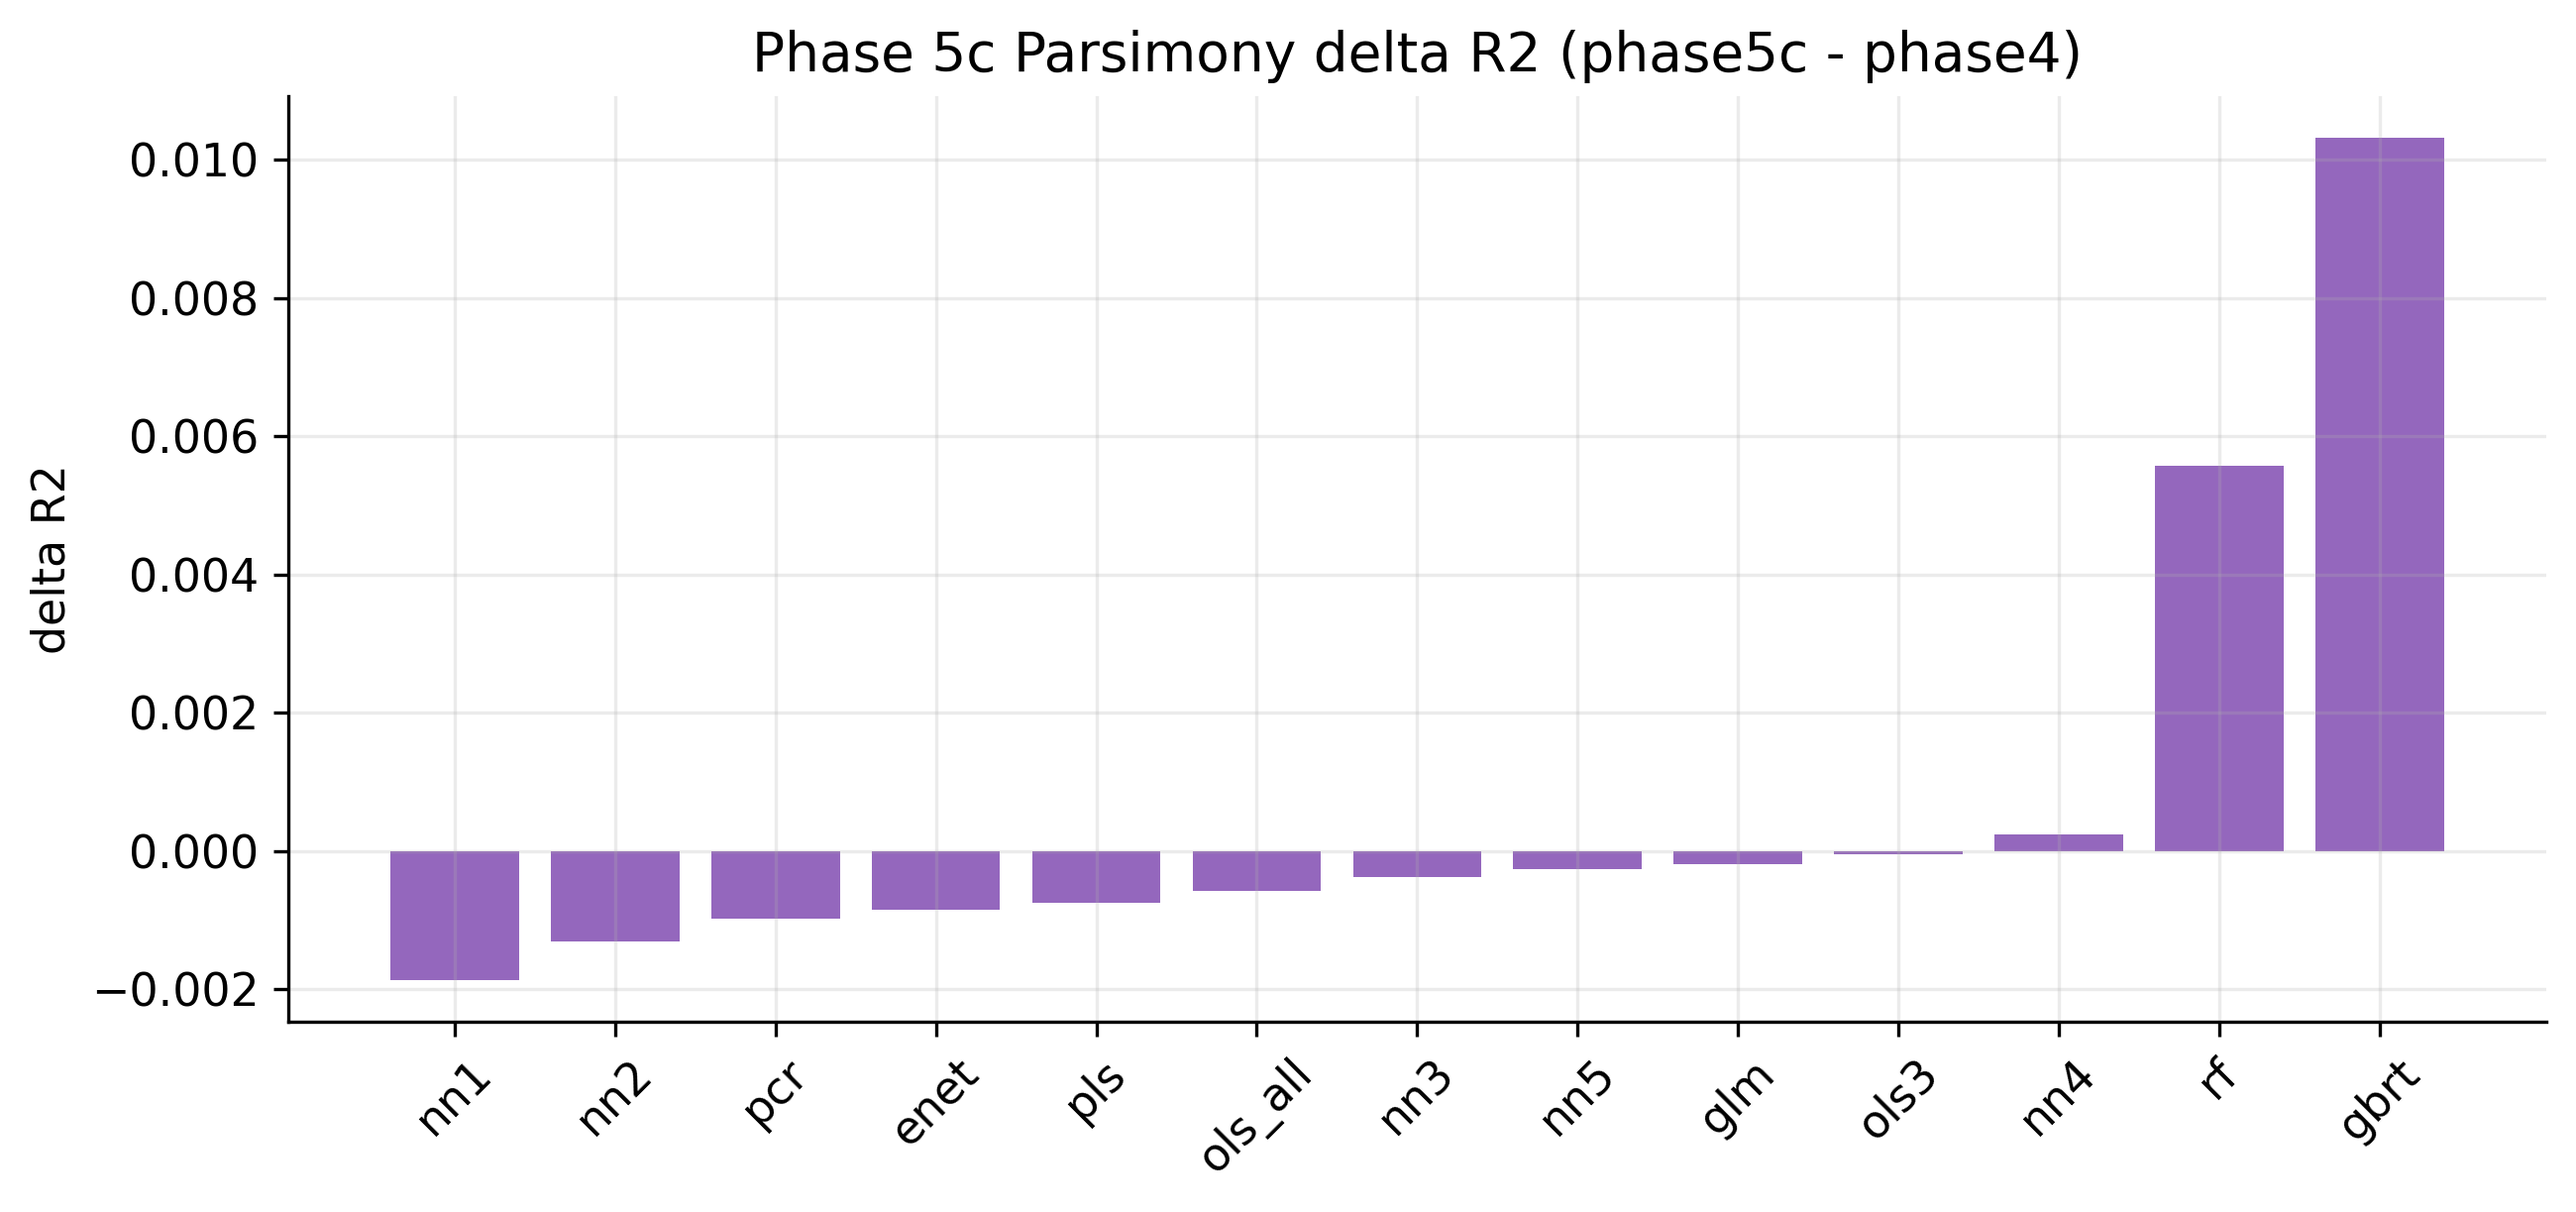
\includegraphics[width=0.85\textwidth]{figures/fig_phase5c_delta_r2.png}
  \caption{Delta OOS $R^2$ (parsimonious minus full-feature) per model. Positive bars: parsimonious outperforms full-feature.}
  \label{fig:delta_r2}
\end{figure}

\subsection{Portfolio Performance (Audited)}

\noindent\small Audited metrics exclude zero-variance prediction months; canonical metrics use all 360 months.

\begin{table}[H]
\centering
\caption{Extension~3: Parsimonious model L/S portfolio performance (audited). NN4: 312/360 non-degenerate months; NN5: 144/360.}
\label{tab:parsimony_port}
\begin{tabular}{lccccccr}
\toprule
Model & Ann. Ret & Ann. Vol & Sharpe & FF5 $\alpha$ & $t_\alpha$ & $p_\alpha$ & Months \\
\midrule
\texttt{nn2} & 0.168 & 0.184 & 0.915 & 0.151 & 4.40 & 0.0000 & 360 \\
\texttt{nn5} & 0.072 & 0.087 & 0.830 & 0.098 & 3.49 & 0.0005 & 144 \\
\texttt{nn1} & 0.171 & 0.213 & 0.801 & 0.154 & 4.61 & 0.0000 & 360 \\
\texttt{pcr} & 0.144 & 0.186 & 0.773 & 0.131 & 3.83 & 0.0001 & 360 \\
\texttt{pls} & 0.136 & 0.191 & 0.709 & 0.135 & 3.67 & 0.0002 & 360 \\
\texttt{ols\_all} & 0.125 & 0.185 & 0.678 & 0.127 & 3.42 & 0.0006 & 360 \\
\texttt{enet} & 0.126 & 0.188 & 0.669 & 0.122 & 3.43 & 0.0006 & 360 \\
\texttt{nn4} & 0.071 & 0.132 & 0.536 & 0.073 & 2.86 & 0.0043 & 312 \\
\texttt{ols3} & 0.090 & 0.170 & 0.527 & 0.085 & 2.69 & 0.0072 & 360 \\
\texttt{glm} & 0.099 & 0.204 & 0.486 & 0.082 & 2.24 & 0.0250 & 360 \\
\texttt{nn3} & 0.042 & 0.117 & 0.362 & 0.045 & 2.45 & 0.0144 & 360 \\
\texttt{gbrt} & 0.047 & 0.185 & 0.255 & 0.039 & 1.05 & 0.2940 & 360 \\
\texttt{rf} & 0.047 & 0.212 & 0.223 & 0.031 & 0.84 & 0.4022 & 360 \\
\bottomrule
\end{tabular}
\end{table}


\subsection{Degenerate Month Audit}
\label{app:parsimony_audit}

\noindent\small NN4: 48 degenerate months (312/360 usable); NN5: 216 degenerate months (144/360 usable, 60\% rate); all other models: 0 degenerate months.

\begin{figure}[H]
  \centering
  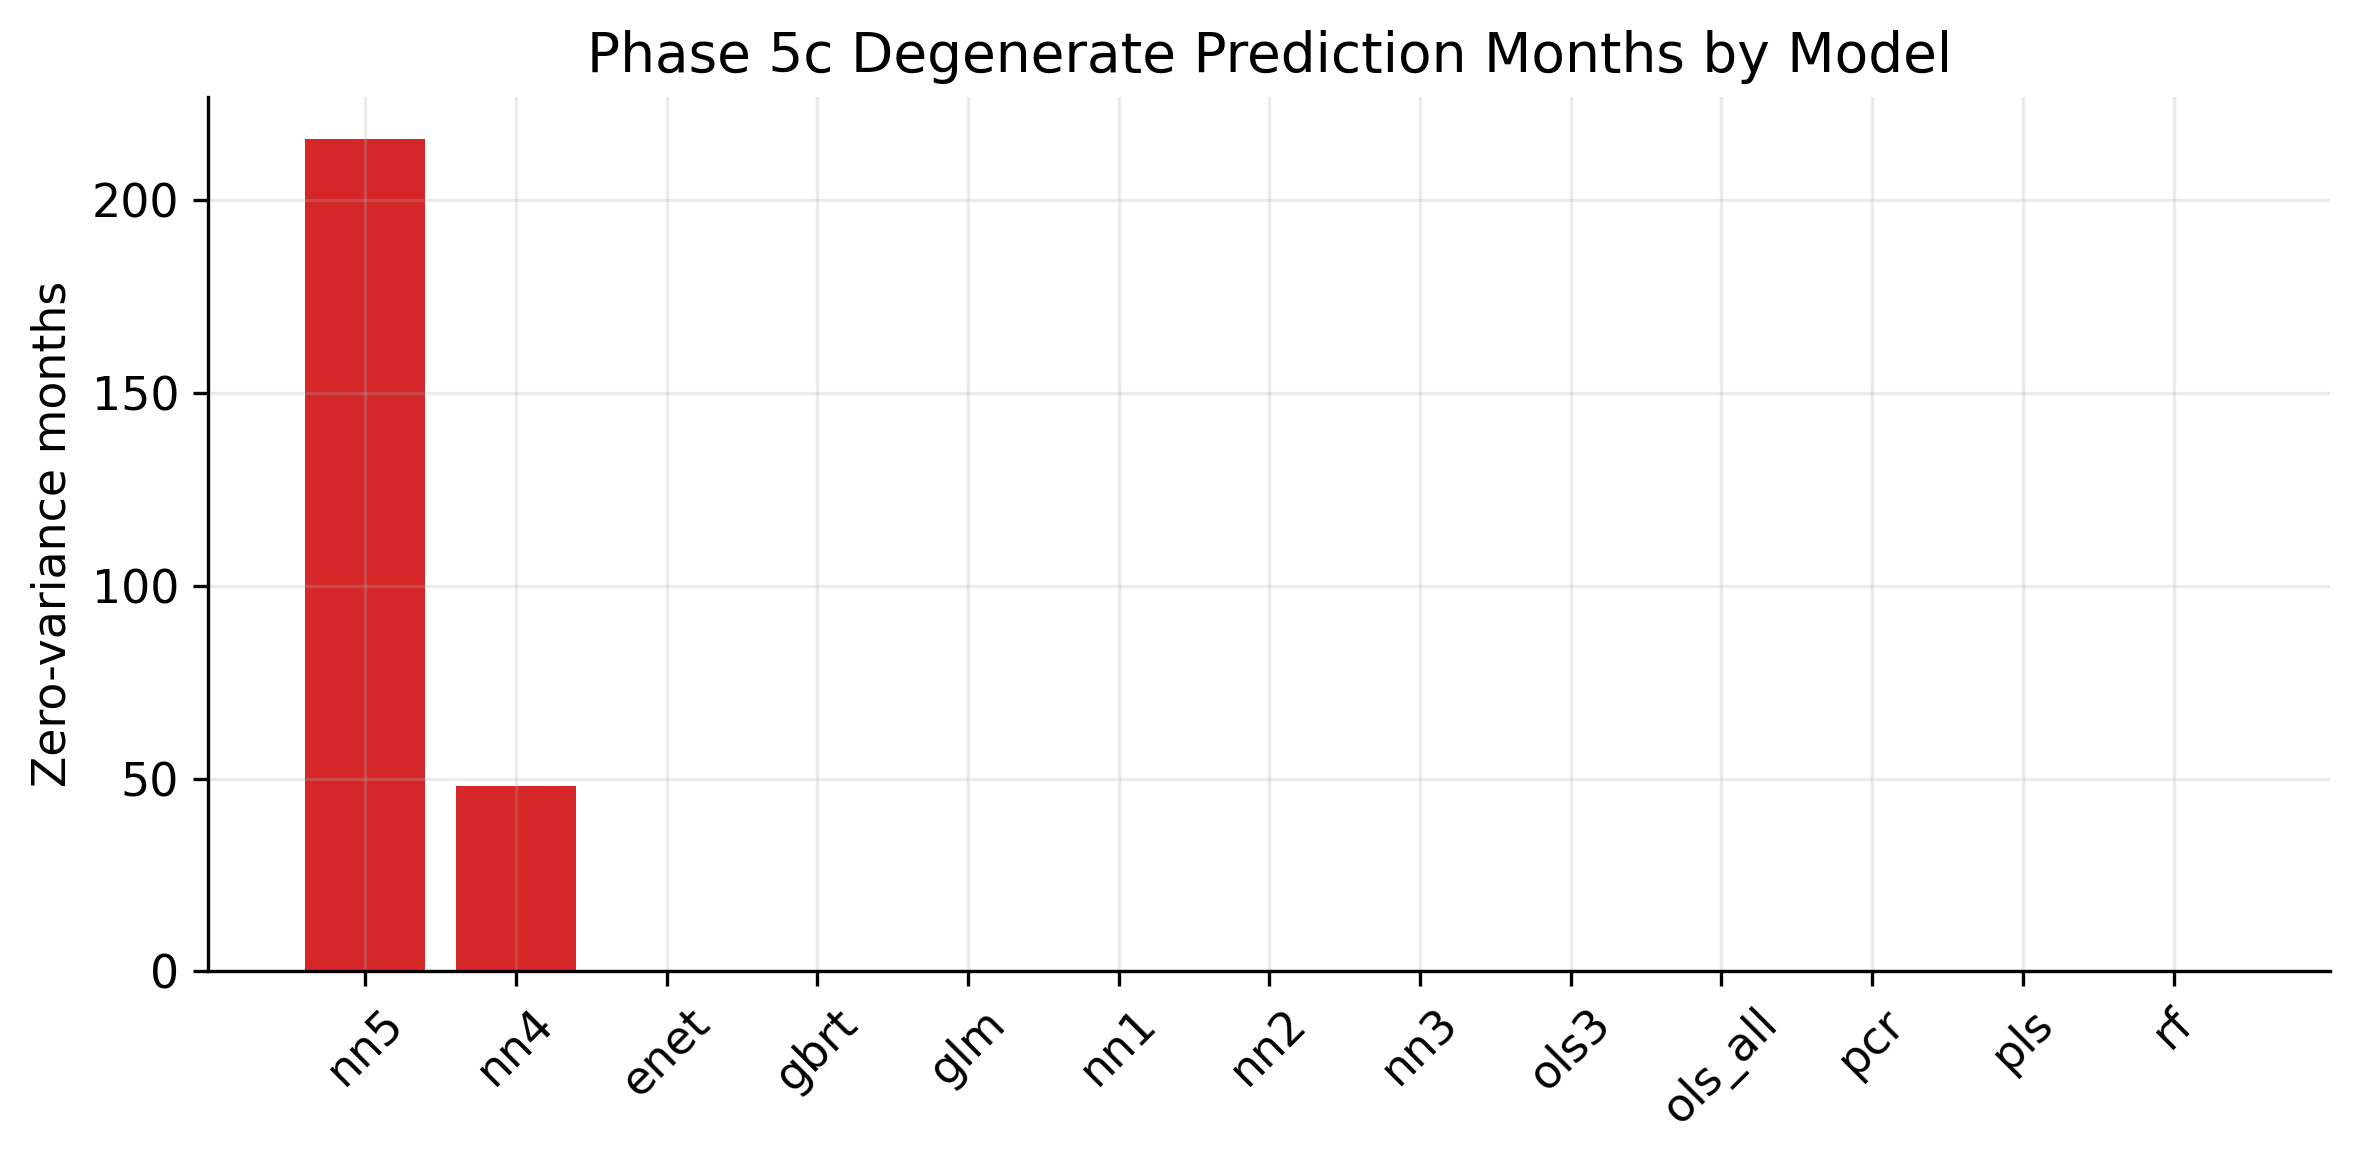
\includegraphics[width=0.85\textwidth]{figures/fig_phase5c_degenerate_months.png}
  \caption{Zero-variance prediction months per model under the parsimonious feature set.}
  \label{fig:degen_months}
\end{figure}

% ============================================================
\section{Data and Pipeline Summary}
\label{app:pipeline}

\subsection{Data Sources}

\noindent\small CRSP monthly file (1957--2024), Compustat annual/quarterly (6- and 3-month public lags), CCM link table, Fama-French 5-factor data.

\subsection{Feature Engineering}

\noindent\small 94 firm characteristics per GKX Table~A.1; cross-sectional rank normalisation to $[-1,+1]$ applied in \texttt{src/features/feature\_assembler.py}.

\subsection{Computational Environment}

\noindent\small All models trained on CPU; Phase~4 wall-clock time $\approx$\,4.7 hours; predictions cached as Parquet files (\texttt{data/processed/predictions.parquet}).

% ============================================================
%  BIBLIOGRAPHY  (after appendix, outside body page count)
% ============================================================
\newpage
\bibliographystyle{apalike}
\bibliography{references}

% ============================================================
%  FUTURE EXTENSIONS AND PRACTICAL CONCLUSION
% ============================================================
\bigskip
\section*{Future Extensions and Code Availability}

The scope of this project is bounded by CPU-only training, a fixed 10-seed ensemble, and a 2024 data horizon. GPU training would allow larger NN ensembles and broader hyperparameter search, while newer data vintages would permit rolling external validation beyond the current cut-off. NLP, ESG, and alternative data are straightforward to integrate in the existing pipeline. The codebase for data assembly, model training, evaluation, and all extensions is maintained privately and available upon request.

% ============================================================
%  END OF DOCUMENT
% ============================================================
\end{document}
